\section{Design of an FPGA-based accelerator integrating structured sparse DSC} \label{sec:design}
As previously said,  the aim of this section is to develop a pruning scheme for \acrshort{cnn} model (MobileNetV2) and a dataflow able to support it. First we details the pruning scheme used and the gain obtained by applying the pruning. 
%
\subsection{Pruning scheme} \label{subsec:pscheme}
%
\acrshort{dsc} is composed of two types of convolution: depthwise and pointwise convolution. We have decided to apply pruning on the pointwise filters for various reasons:
%
\begin{itemize}
    \item In MobileNet and MobileNetV2, most of the operations are done in the pointwise convolutions \cite{zhang_channel_2019, tu_pruning_2019}.
    \item As each kernel of pointwise kernel, is a vector of size $1 \times 1  \times Nif$. It means that we have to prune in the axis of the channel and apply the same scheme as \textcite{kang_accelerator-aware_2020}.
    \item As in MobileNetV2, each \acrshort{dsc} follows a $1 \times 1$ convolution, we can apply the pruning scheme to every $1 \times 1$ convolutions in the network.
\end{itemize}
%
As mentionned above, we can develop a pruning scheme that is inspired by the methodology of \textcite{kang_accelerator-aware_2020} which performs an channel-axis pruning. Ideally, without pruning, each \acrshort{pe} performing a pointwise convolution, fetches $N_{if}$ weights and their corresponding input pixels (pointwise convolution only convolve pixels in the channel-axis). Then each non-pruned weight is convolved with its corresponding pixel. However, as the resource of the \acrshort{fpga} are limited, the \acrshort{pe} can load $N_{par} \leq N_{if}$ weights and pixels.

%
\begin{figure}
    \centering
    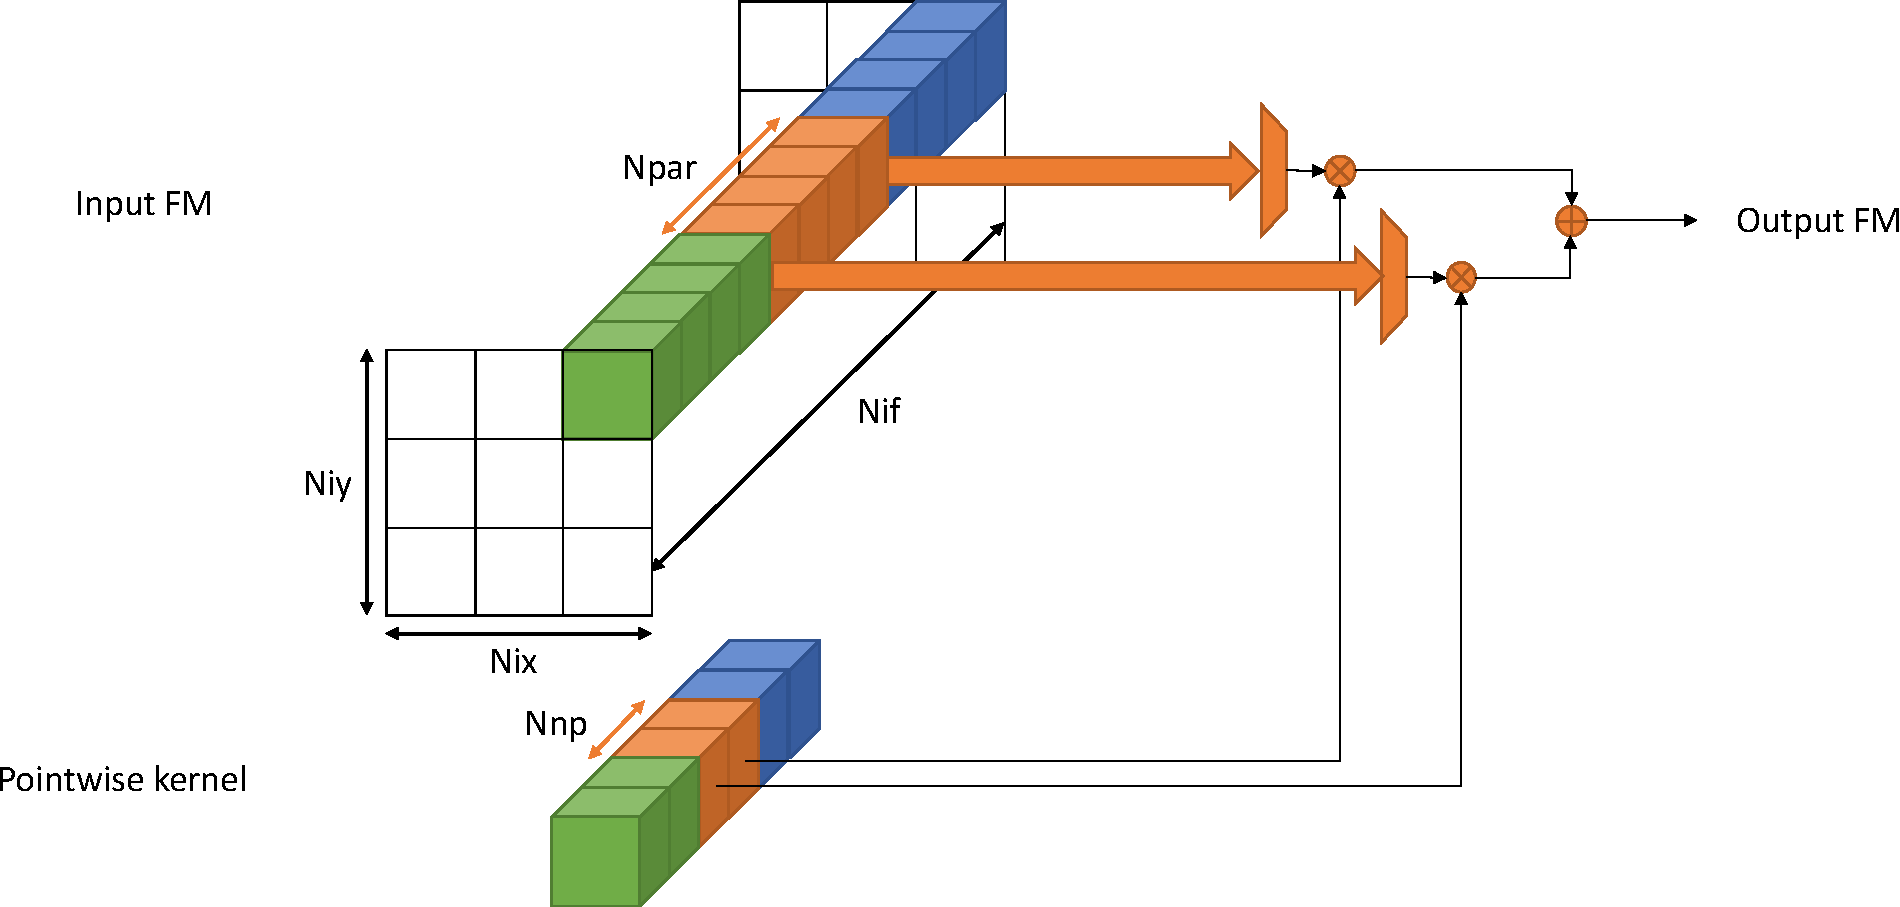
\includegraphics[width=\textwidth]{pruningscheme.pdf}
    \caption{Process of convolution with a sparse pointwise kernel, inspired from \cite{kang_accelerator-aware_2020}}
    \label{fig:prunedwg}
\end{figure}
%
As pointed out by \cite{kang_accelerator-aware_2020}, the unstructured pruning of the pointwise kernel can cause several issues. First, it can causes misalignement between the weight and pixel fetching group. Indeed if we prune the first $N_{par}$ weights in the kernel, the first pixels fetching is useless. Second, there can be a load-imbalance problem that can occur between two \acrshort{pe}s if the number of weights between the two kernels is different. To solve these problems, the solution proposed by \cite{kang_accelerator-aware_2020} is to allign fetching groups of size $N_{par}$, and for each weight fetching group keep a uniform number of weights called $N_{np}$, as illustrated in Figure \ref{fig:prunedwg}. Therefore, it solves also the load imballance problem and can be applied to every $1 \times 1$ kernels.

%
\begin{table}
    \center
    \begin{tabular}{|c|c|c|}
        \hline
        $N_{par}$ & The input pixel fetching group size. & $N_{par} \leq N_{if}$ \\
        \hline
        $N_{np}$  & The pointwise weight fetching group size. & $N_{np} \leq N_{par}$ \\
        \hline
        $N_{gr}$  & The number of fetching groups & $N_{gr} = \left\lceil \frac{N_{if}}{N_{par}} \right\rceil $ \\
        \hline
        $\alpha$  & The pruning ratio & $\alpha = \frac{N_{np}}{N_{par}}  $ \\
        \hline
    \end{tabular}
    \caption{Pruning parameters}
    \label{tab:pr_param}
\end{table}
%
To summarise, each depthwise kernel is composed of $N_{gr}$ weight fetching groups of $N_{np}$ weights, where each group corresponds to a pixels fetching group of size $N_{par}$. We should add that this pruning scheme is not the same as \textit{channel pruning} since we do not constraint the same weights to be pruned in each group. Therefore, I have not considered the pruning of the pointwise filter associated with the pruning of a weight in each kernels. The pruning parameters are defined in Table \ref{tab:pr_param}.
%
\subsubsection{Reduction factor}
%
We can now evaluate the reduction factor of the \acrshort{dsc} including pruning with respect to the \acrshort{dsc} without pruning and the standard convolution. Considering the size of the input feature map of the pointwise convolution is $N_{ix}  \times N_{iy} \times N_{if}$, the size of the depthwise filter is $N_{kx} \times N_{ky} \times N_{if}$, the size of the non-pruned pointwise convolution $N_{if} \times N_{of}$, the fetching group size is $N_{par}$, and the number of pruned weights is $N_{np}$. The amount of weights $W_{DSC}$ and operations $O_{DSC}$ of the \acrshort{dsc} can be determined using Equation \eqref{eq:dsc_wg_op} \cite{bai_cnn_2018, liu_fpga-based_2019}.
%
\begin{align}
    W_{DSC} &= N_{kx} \times N_{ky} \times N_{if} + N_{if} + \times N_{of}\\
    O_{DSC} &= N_{ix} \times N_{iy} \times N_{kx} \times N_{ky} \times N_{if} + N_{ix} \times N_{iy} \times N_{if} \times N_{of}
    \label{eq:dsc_wg_op}
\end{align}
%
The same way, the amount of weights $W_{PR_DSC}$ and operations $O_{PR_DSC}$ of the \acrshort{dsc} with pruning can be determined using Equation \eqref{eq:pr_dsc_pr_wg_op}.
%
\begin{align}
    W_{PR_DSC} &= N_{kx} \times N_{ky} \times N_{if} + \times N_{if} + N_{np} \times N_{gr} \times N_{of}\\
    O_{PR_DSC} &= N_{ix} \times N_{iy} \times N_{kx} \times N_{ky} \times N_{if} + N_{ix} \times N_{iy} \times N_{gr} \times N_{np} \times N_{of} 
    \label{eq:pr_dsc_wg_op}
\end{align}
%
Thus, the reduction factor on weights $F_{Wg}$ and operations $F_{Op}$ can be calculated in Equation \eqref{eq:factor_comp}. More information about the demonstration to find the relations can be found in Appendix \ref{appendix:factor}.
%
\begin{align}
    F_{Wg} &= \frac{1 + \frac{N_{kx} \times N_{ky}} {N_{of}}} {\alpha + \frac{N_{kx} \times N_{ky}} {N_{of}}}\\
    F_{Op} &= \frac{1 + \frac{N_{kx} \times N_{ky}} {N_{of}}} {\alpha + \frac{N_{kx} \times N_{ky}} {N_{of}}}
    \label{eq:factor_comp}
\end{align}
%
\begin{figure}
    \centering
    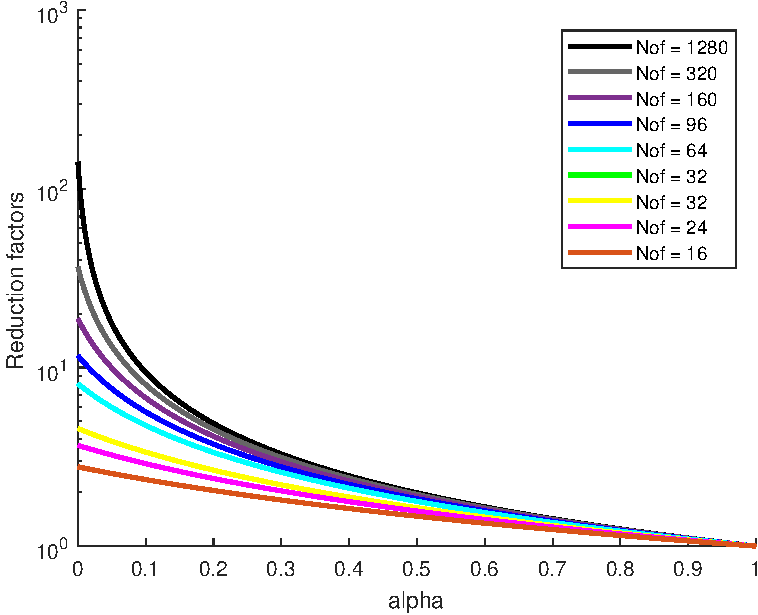
\includegraphics[width=\textwidth]{RedFactor.pdf}
    \caption{Evolution of the reduction factor depending on the pruning ratio and the number of output channel}
    \label{fig:redfacto}
\end{figure}
%
As the reduction factor depend on the pruning ratio $\alpha$, we can illustrate the evolution of the reduction factors depending on this parameter and on the different $N_{of}$ of the network. This can be seen on Figure \ref{fig:redfacto}. For example, if we apply a pruning ratio of $75\%$, the reduction factors with respesct to the \acrshort{dsc} without pruning are between two and four times. If we consider the reduction factor between \acrshort{dsc} and standard convolution to be 9 times, the reduction factors between proposed \acrshort{dsc} and standard convolution is between 18 and 36 times
%
\subsubsection{Compressed format}
%
\begin{figure}
    \centering
    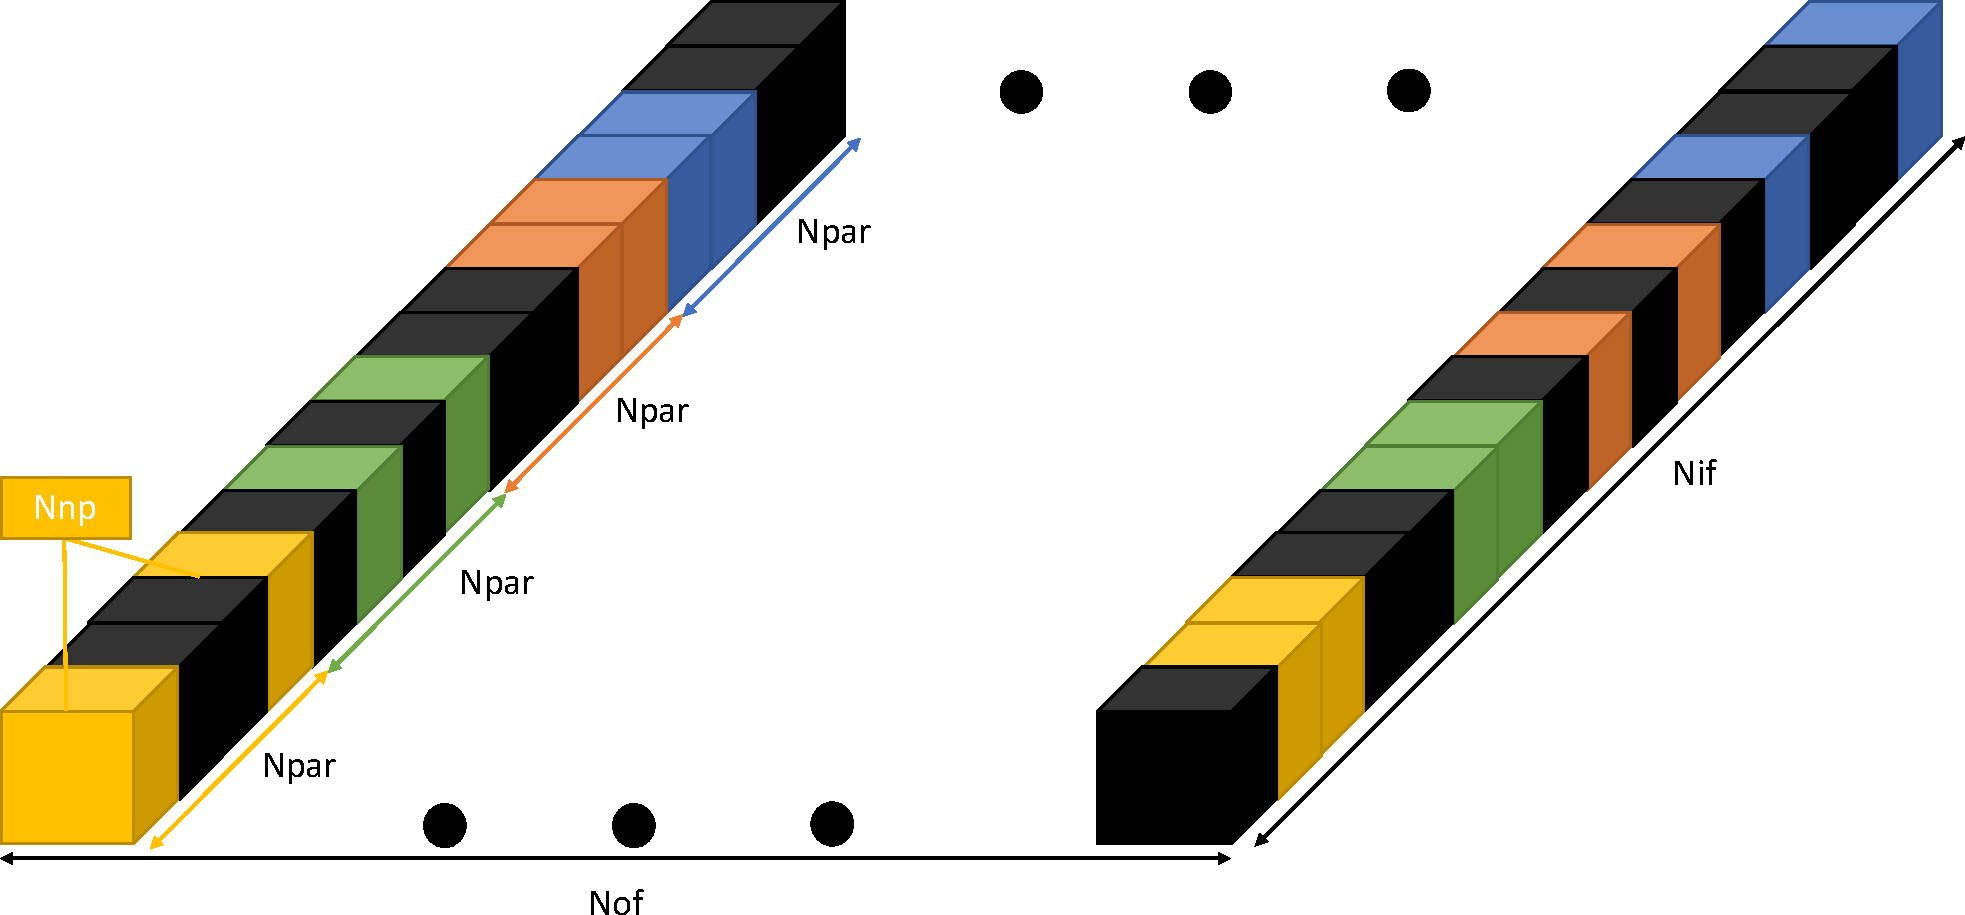
\includegraphics[width=\textwidth]{pruned_wg.pdf}
    \caption{A pointwise kernel after pruning}
    \label{fig:pruned_wg}
\end{figure}
%
After applying the pruning scheme on the pointwise kernels, the kerels become sparse and it means that is contains a lot of 0 value weights, as illustrated in Figure \ref{fig:pruned_wg}. Therefore, in order to reduce the memory usage, we should store the non-pruned weights in a compressed format that allow to find the address of the weight with no extra-overhead.

A conventional storage formats for sparse matrix is the \acrfull{csr} \cite{buluc_parallel_2009}. According to \textcite{buluc_parallel_2009}, \textquote{\textit{The compressed sparse row (CSR) format stores the nonzeros (and ideally only the nonzeros) of each matrix row in consecutive memory locations,  and  it  stores  an  index  to  the  first  stored  element of each row}}. In other words, we represent a sparse matrix using three vectors:
%
\begin{itemize}
    \item \textbf{Vector val}: containing all the values of the non-pruned weights.
    \item \textbf{Vector col\_ind}: contains the column indices of the elements in \textbf{val}.
    \item \textbf{Vector row\_ptr}: contains the index of each row in \textbf{val}.
\end{itemize}
%
However, as for \cite{zhu_efficient_2020}, this format can be compressed further thanks to the pruning scheme. Indeed, since the kernels to compress are vectors, we can reduce the storage usage by removing the \textbf{row\_ptr} vector. Moreover, we have a better compression if we reduce the number of bits allocated to represent the column index of a weigth. Indeed, knowing that the weight correpond to a pixel in a fetching group of size $N_{par}$, we can only save the position of the pixel in that group. As a result, we can reduce the number of bits from $log_2(N_{if})$ to $log_2(N_{par})$, where $N_par \leq N_{if}$.

%
\begin{figure}
    \centering
    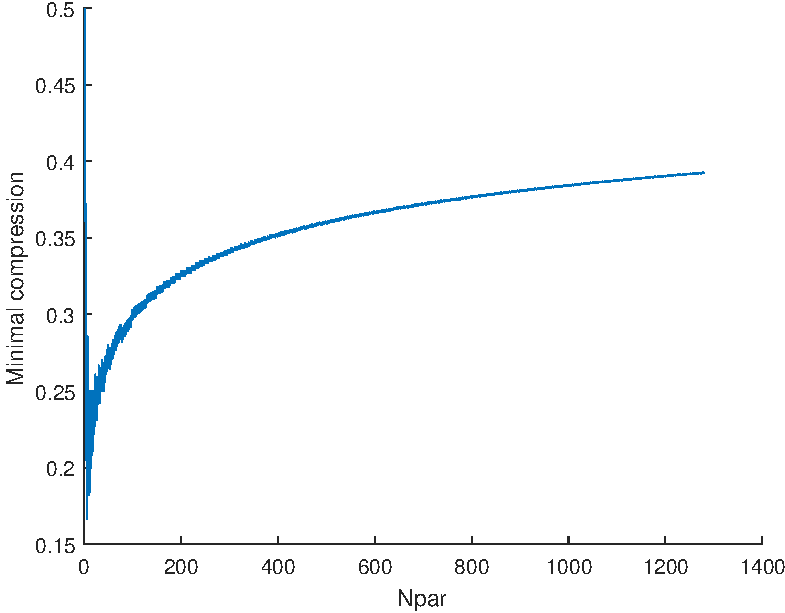
\includegraphics[width=\textwidth]{MinCompr.pdf}
    \caption{Minimal pruning ratio if $BW$ = 16}
    \label{fig:prun_mem}
\end{figure}
%
As this compressed format requires an extra vector, we compute the minimal pruning ratio required to have a reduction of the memory usage. The relation between minimal pruning ratio and memory reduction ca be found in Equation \eqref{eq:prun_mem} where $BW$ is the bitwidth required to represent the value of a weight. The curve representing the minimal pruning ratio depending on $N_{par}$ is illustrated in Figure \ref{fig:prun_mem}. We can conclude that we need at least a pruning ration of $40\%$ in order to save memory (a fewer pruning ratio can be set if we have a small $N_{par}$).
% 
\begin{equation}
    \alpha < \frac{BW}{ BW + log_2(N_{par})}
    \label{eq:prun_mem}
\end{equation}
%
\subsection{Adding the pruning scheme to MobileNetV2}
%
As we have seen how the weights of a $1 \times 1$ kernel are pruned and the compressed format of the kernels, we explain in this section how to integrate the proposed pruning scheme into the \acrshort{dsc}. In MobileNetV2, the \acrshort{dsc} layer is included into a larger building block, the \textit{inverted residual block} (see Section \ref{subs:mbv2}). It means that the \acrshort{dsc} follows a $1 \times 1$ convolution layer that expands the number of channel. As a result, we have to compute two sparse $1 \times 1$ convolutions. 

%
\begin{figure}
    \centering
    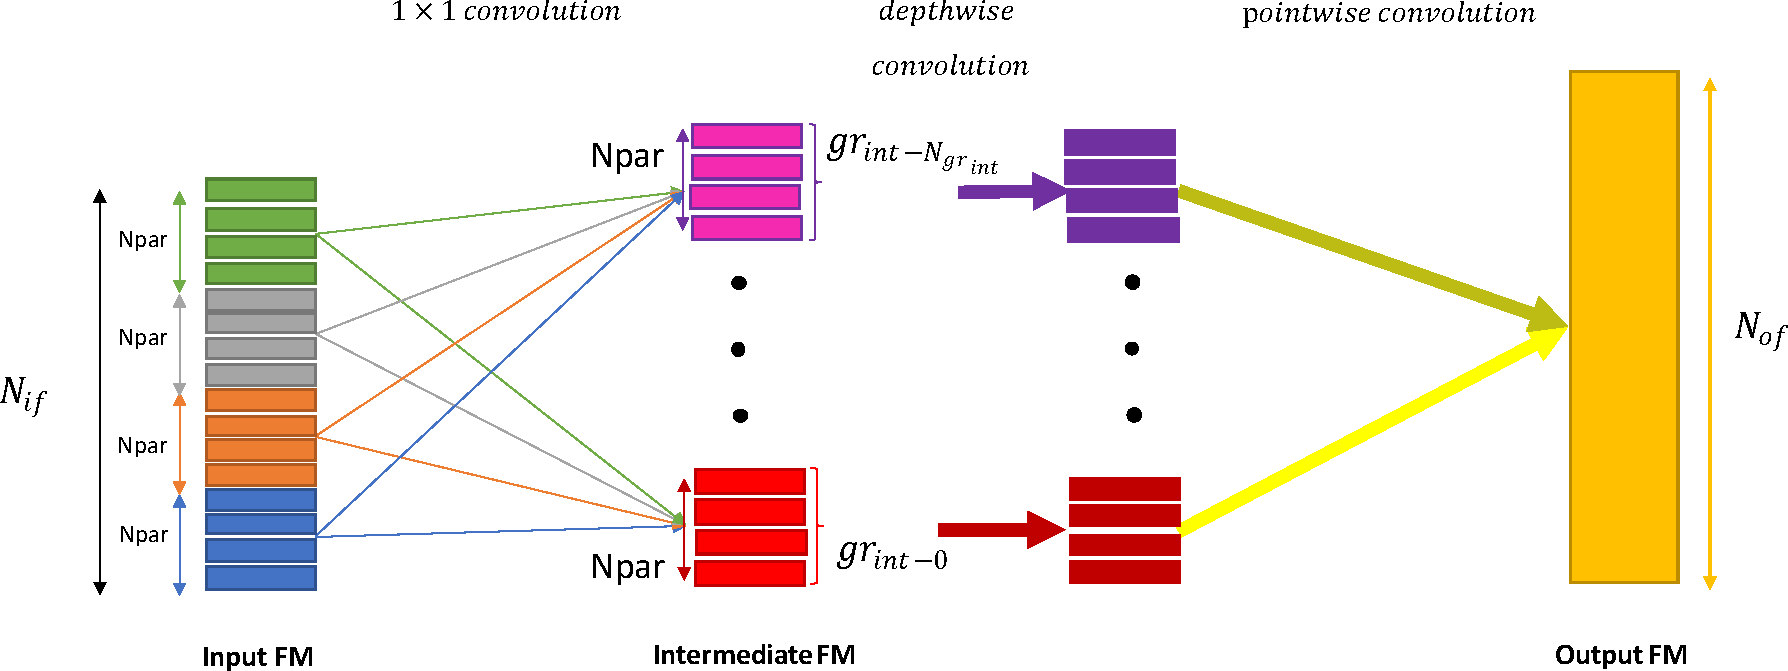
\includegraphics[width=\textwidth]{algo.pdf}
    \caption{Illustration of the algorithm used to perfom the convolutions}
    \label{fig:algo}
\end{figure}
%
As explained in Section \ref{subsec:pscheme}, each $1 \times 1$ convolution has to fetch $N_{par}$ input pixels, which corresponds to $N_{par}$ channels. Consequently, if the expansion $1 \times 1$ convolution produces $N_{par}$ channels, the \acrshort{dsc} can fetches those intermediate products and produces partial results of the output \acrshort{fm}. Indeed, we can first perform the depthwise convolution with each intermediate channel and then performing the partial pointwise convolution with the corresponding weight in each pointwise kernel, as illustrated in Figure \ref{fig:algo}. The block has finished when it has performed the previous steps for each intermediate group. This approach has been chosen, instead of producing directly each final output result, to reuse at most the products of the $1 \times 1$ convolution.

\begin{algorithm}[H]
    \centering
    \begin{algorithmic}
        \For{$group_{int}:=0$; $group_{int} < Ngr_{int}$; $group_{int}++$}
            \State{1*1\_convolution ($group_{int}$)}
            \State{DSC($group_{int}$);}
        \EndFor
    \end{algorithmic}
    \caption{Pseudocode of the algorithm}
    \label{pseudocode:overal_pseudo_code}
\end{algorithm}
%
We can translate this algorithm into a pseudocode, observed at Figure \ref{pseudocode:overal_pseudo_code}, where $group$ (respect. $group_{int}$) is the index of fetching group in the input \acrshort{fm} (resp. intermediate \acrshort{fm}, since the number of input channels is expanded by a factor $t$) and $Ngr_{int} = \left\lceil \frac{N_{if} \times t}{N_{par}} \right\rceil$ is the number of intermediate fetching group. We can now detail how each convolution is going to be performed:
%
%
\begin{enumerate}
    \item \textbf{1*1\_convolution}: We have to fetch the $N_{par}$ kernels corresponding to the \acrshort{dsc} fetching group. Indeed, the \acrshort{dsc} fetches $N_{par}$ channels corresponding to a spatial position $(intx, inty)$ of the intermediate \acrshort{fm}. Then we can perform the convolution. As described in Section \ref{subs:2dconv}, the kernel acts a sliding window on the input \acrshort{fm}. For each pixel at position $(ix, iy)$, the convolution loads iteratively each weight and pixel fetching group. For each fetching group $group \leq N_{group}$, the convolution is performed by multiplying each non-pruned weight with its corresponding channel and accumulates it with the result of the previous group. The process is finished when the $N_{par}$ intermediate \acrshort{fm} channels have been produced (of size $N_{ix} \times N_{iy}$). The corresponding pseudocode is found in Algorithm \ref{pseudocode:c11} and the process is shown in Figure \ref{fig:algo_11conv}.
    \begin{algorithm}[H]
        \centering
        \begin{algorithmic}
            \For{$int_{f}:=0$; $int_{f} < N_{par}$; $int_{f}++$} \Comment{Loop 3}
                \For{$int_{x}:=0$; $int_{x} < N_{ix}$; $int_{x}++$} \Comment{Loop 2}
                    \For{$int_{y}:=0$; $int_{y} < N_{iy}$; $int_{y}++$} \Comment{Loop 2}
                        \For{$group:=0$; $group < N_{gr}$; $group++$} \Comment{Loop 1}
                            \For{$i_f:=0$; $i_f < N_{np}$; $i_f++$} \Comment{Unrolled}
                                \State{$wgt$  = $filter_{1 \times 1}$[$group_{int} \times N_{par} + int_f$][$group \times N_{par} + i_f$]}
                                \State{$acti$  = $FMI_{I}$[$wgt[pos] + group \times N_{par}$][$int_y$][$int_x$]}
                                \State{FM$_{int}$[$group_{int} \times N_{par} + int_f$][$int_y$][$int_x$]  += $acti \times wgt[val]$}
                            \EndFor
                        \EndFor
                    \EndFor
                \EndFor
            \EndFor
        \end{algorithmic}
        \caption{Sparse $1 \times 1$ convolution pseudocode}
        \label{pseudocode:c11}
    \end{algorithm}
    %
    \begin{figure}[H]
        \centering
        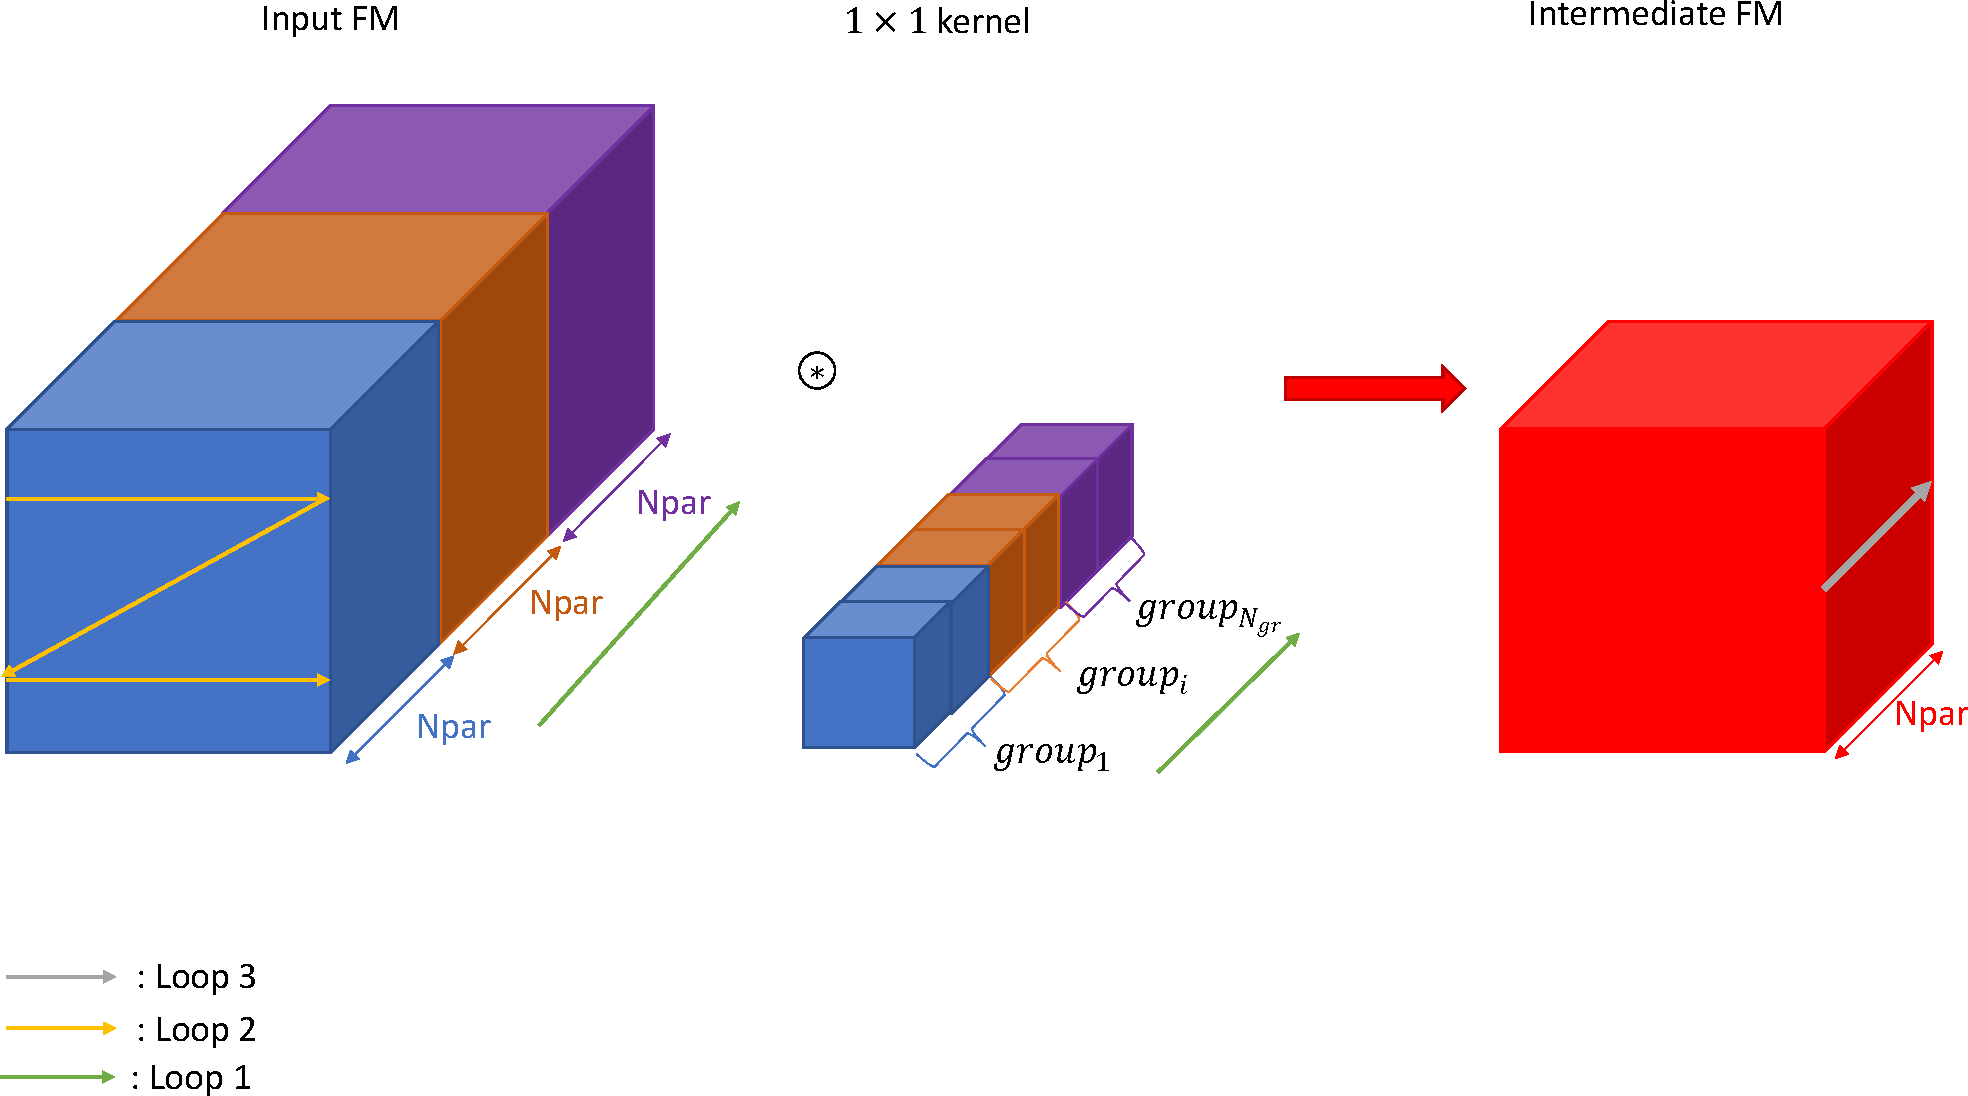
\includegraphics[width=\linewidth]{algo_c11.pdf}
        \caption{representation of the sparse $1 \times 1$ convolution}
        \label{fig:algo_11conv}
    \end{figure}
    %
    \item \textbf{\acrshort{dsc}} Once the $1 \times 1$ convolution has produced the next $N_{par}$ input channels of the \acrshort{dsc}, we can first do the depthwise convolution on the intermediate \acrshort{fm}. Once the depthwise convolution is done, we can fetch the corresponding weight fetching group in each of the pointwise filters and compute the partial results for each of the output \acrshort{fm}. The corresponding pseudocode is found in Algorithm \ref{pseudocode:dsc} and the process is shown in Figure \ref{fig:algo_dsc}.
    %
    \begin{algorithm}[H]
        \centering
        \begin{algorithmic}
            \For{$int_{f}:=0$; $int_{f} < N_{par}$; $int_{f}++$} \Comment{Loop 3}
                \For{$int_{x}:=0$; $int_{x} < N_{ix}$; $int_{x}++$} \Comment{Loop 2}
                    \For{$int_{y}:=0$; $int_{y} < N_{iy}$; $int_{y}++$} \Comment{Loop 2}
                        \For{$group:=0$; $group < N_{gr}$; $group++$} \Comment{Loop 1}
                            \For{$i_f:=0$; $i_f < N_{np}$; $i_f++$} \Comment{Unrolled}
                                \State{$wgt$  = $filter_{1 \times 1}$[$group_{int} \times N_{par} + int_f$][$group \times N_{par} + i_f$]}
                                \State{$acti$  = $FMI_{I}$[$wgt[pos] + group \times N_{par}$][$int_y$][$int_x$]}
                                \State{FM$_{int}$[$group_{int} \times N_{par} + int_f$][$int_y$][$int_x$]  += $acti \times wgt[val]$}
                            \EndFor
                        \EndFor
                    \EndFor
                \EndFor
            \EndFor
        \end{algorithmic}
        \caption{Sparse \acrshort{dsc} convolution pseudocode}
        \label{pseudocode:dsc}
    \end{algorithm}
    %
    \begin{figure}[H]
        \centering
        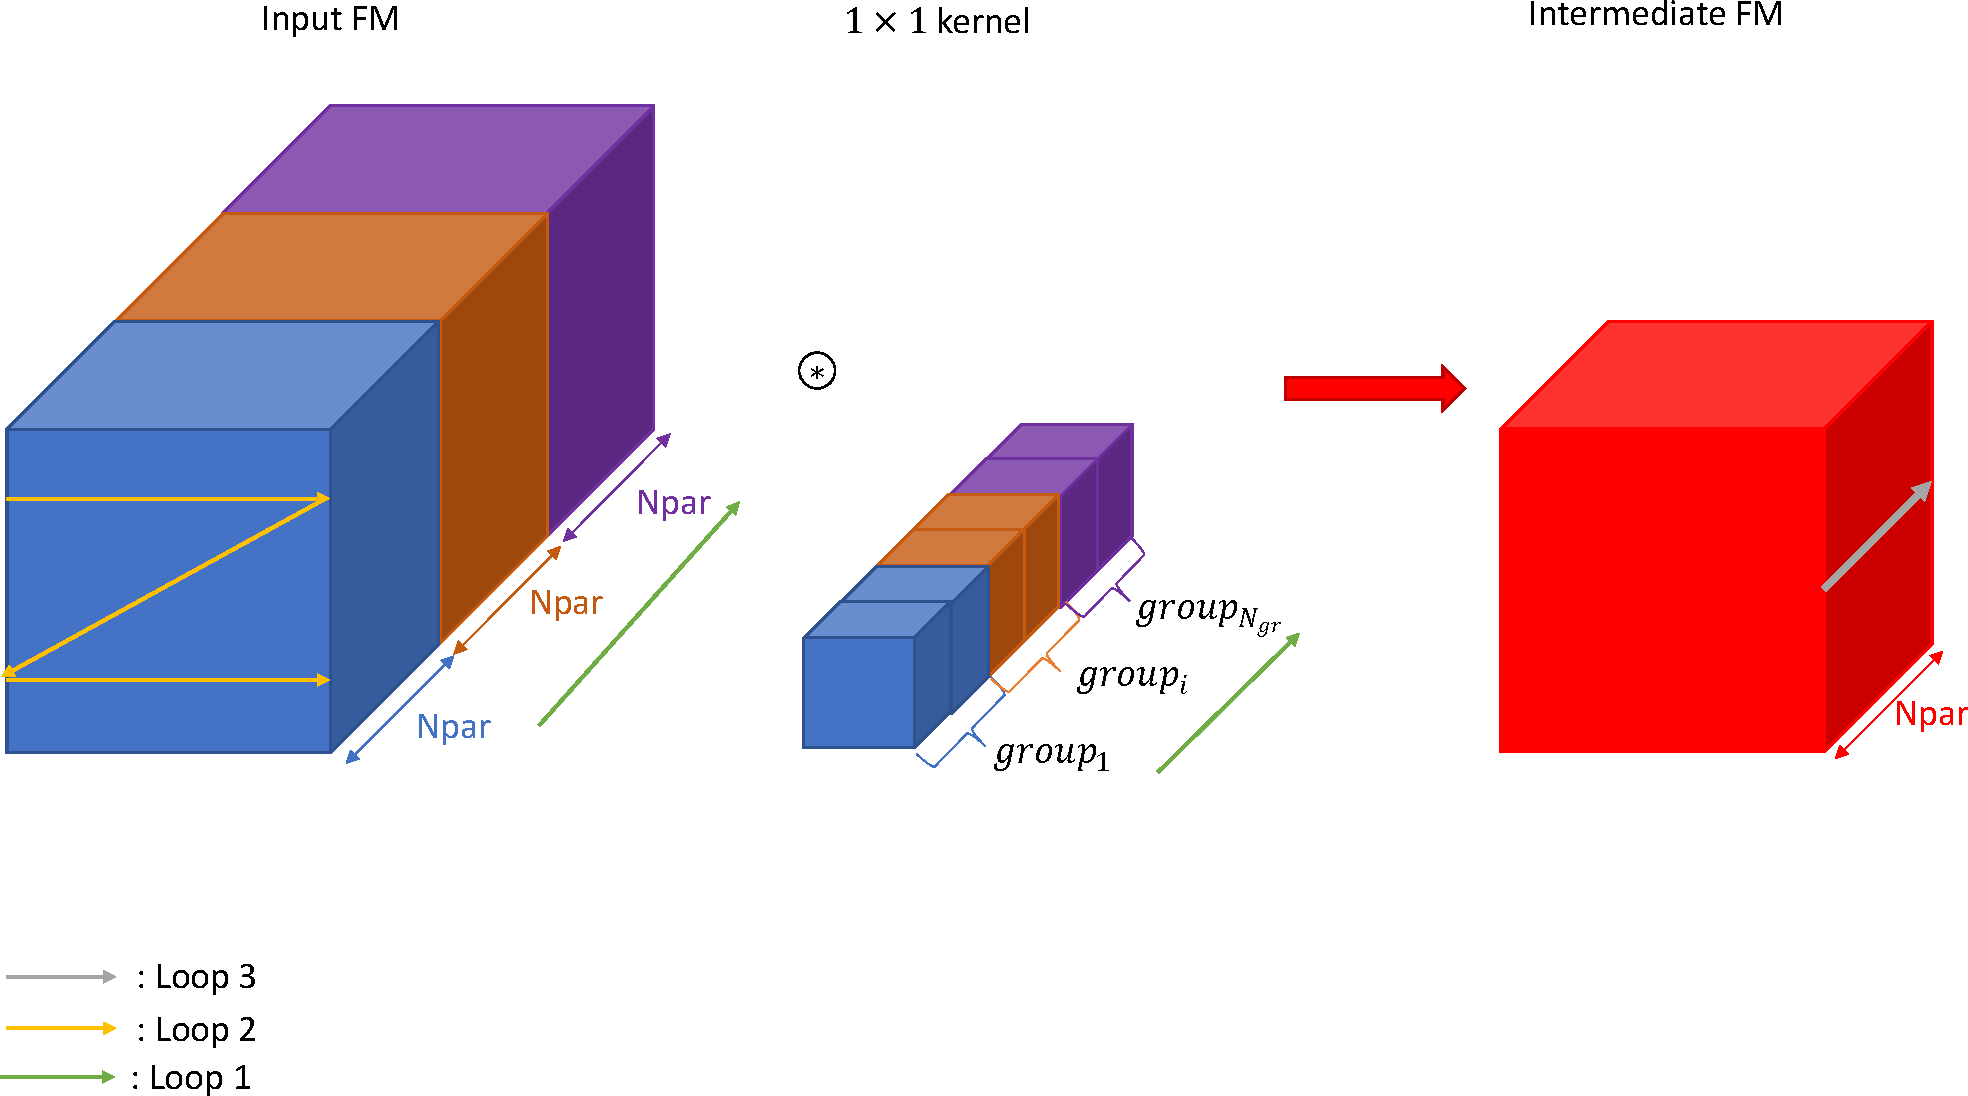
\includegraphics[width=\linewidth]{algo_c11.pdf}
        \caption{representation of the sparse \acrshort{dsc} convolution}
        \label{fig:algo_11conv}
    \end{figure}
\end{enumerate}
%
\subsection{Loop analysis}
%
Once we have determined how the convolutions is going to be performed
on \acrshort{fpga}, now we have to analyse the loop in order to find the optimal tiling, unrolling and loop interchange parameters.